\begin{exo}{}
	Associer à chaque tableau de variations sa la courbe représentation.

	\begin{enumerate}
		\item
		      \begin{tikzpicture}
			      \tikzset{arrow style/.style={->, >=Triangle, thick}}
			      \tikzset{double style/.style={double, line width=1pt, double distance=2pt, draw=black}}
			      \tkzTabInit[lgt=1.5,espcl=2]{$x$ / 0.7 , $f_1$ / 1.3}{$-\infty$, $0$, $+\infty$}
			      \tkzTabVar{-/ , +D-/ , +/ }
		      \end{tikzpicture}

		\item
		      \begin{tikzpicture}
			      \tikzset{arrow style/.style={->, >=Triangle, thick}}
			      \tkzTabInit[lgt=1.5,espcl=4]{$x$ / 0.7 , $f_2$ / 1.3}{$-\infty$, $+\infty$}
			      \tkzTabVar{-/ , +/ }
		      \end{tikzpicture}

		\item
		      \begin{tikzpicture}
			      \tikzset{arrow style/.style={->, >=Triangle, thick}}
			      \tkzTabInit[lgt=1.5,espcl=2.1]{$x$ / 0.7 , $f_3$ / 1.3}{$-\infty$, $2$, $+\infty$}
			      \tkzTabVar{-/ , +/ $3$ , -/ }
		      \end{tikzpicture}

		\item
		      \begin{tikzpicture}
			      \tikzset{arrow style/.style={->, >=Triangle, thick}}
			      \tkzTabInit[lgt=1.5,espcl=1.6]{$x$ / 0.7 , $f_4$ / 1.3}{$-\infty$, $2$, $4$, $+\infty$}
			      \tkzTabVar{-/ , +/ $3$ , -/ $1.5$ , +/ }
		      \end{tikzpicture}
	\end{enumerate}

	\begin{center}
		\begin{tikzpicture}[scale=0.65]
			\draw[color=cyan!30, thin, step=1] (-3.5,-4.5) grid (6.5,4.5);
			\draw[->, >=Triangle, thick] (-3.5,0) -- (6.5,0) node[above left] {$x$};
			\draw[->, >=Triangle, thick] (0,-4.5) -- (0,4.5) node[below right] {$y$};
			\foreach \x in {-3, 1, 5}
			\draw (\x,2pt) -- (\x,-2pt) node[below, font=\small] {$\x$};
			\draw (0,2pt) -- (0,-2pt) node[below, font=\small] {$0$};
			\foreach \y in {-4, 1, 2, 4}
			\draw (2pt,\y) -- (-2pt,\y) node[left, font=\small] {$\y$};
			\foreach \x in {-2, -1, 2, 3, 4, 6}
			\draw (\x,2pt) -- (\x,-2pt);
			\foreach \y in {-3, -2, -1, 3}
			\draw (2pt,\y) -- (-2pt,\y);
			\clip (-3.5,-4.5) rectangle (6.5,4.5);

			% 1. Courbe bleue (croissante, asymptote verticale à gauche)
			\draw[color=blue!70!cyan, line width=1pt, domain=-3.45:6.5, samples=100]
			plot (\x, {1.2*ln(\x+3.5) + 1.5});

			% 2. Courbe rose/violette (croissante à gauche, asymptote verticale vers x=0)
			\draw[color=purple,  line width=1pt, domain=-3.5:-0.2, samples=100]
			plot (\x, {e^(\x+2.2) - 1.5});
			\draw[color=purple, line width=1pt, domain=0.2:6.5, samples=100]
			plot (\x, {2.5*ln(\x) - 1.5});

			% 3. Courbe orange (croissante jusqu'à (2,3) avec un point anguleux puis décroissante)
			\draw[color=orange,  line width=1pt, domain=-3.5:2, samples=100]
			plot (\x, {3 - 2*sqrt(abs(2-\x))});
			\draw[color=orange, line width=1pt, domain=2:6.5, samples=100]
			plot (\x, {1.2 + 1.8/(\x-1)});

			% 4. Courbe verte (maximum local à (2,3) et minimum local à (4,2))
			\draw[color=green!60!black,  line width=1pt, domain=-1.2:5.4, samples=100]
			plot(\x,{9*(1.0/3.0*(\x)^(3.0)-3.0*(\x)^(2.0)+8.0*(\x))/8-4.5});
			\fill (2,3) circle (2pt);
			\fill (4,1.5) circle (2pt);
			\node[blue,above left] at (-1.8,2) {$\mathcal{C}_A$};
			\node[purple,below] at (1.2,-2) {$\mathcal{C}_B$};
			\node[orange,below] at (-2,-1.1) {$\mathcal{C}_C$};
			\node[green!60!black,left] at (5.1,3) {$\mathcal{C}_D$};

		\end{tikzpicture}

	\end{center}


\end{exo}
